\documentclass[UTF8]{ctexart}
\usepackage{geometry}
\usepackage{listings}
\usepackage{xcolor}
\usepackage{graphicx}
\usepackage{float}
\usepackage{multirow}
\usepackage{array}
\usepackage{longtable}
\usepackage{hyperref}
\usepackage{ctex}

\geometry{a4paper,scale=0.8}
\lstset{
    numbers=left, %设置行号位置
    numberstyle=\tiny, %设置行号大小
    keywordstyle=\color{blue}, %设置关键字颜色
    commentstyle=\color[cmyk]{1,0,1,0}, %设置注释颜色
    frame=single, %设置边框格式
    escapeinside=``, %逃逸字符(1左面的键),用于显示中文
    breaklines, %自动折行
    extendedchars=false, %解决代码跨页时,章节标题,页眉等汉字不显示的问题
    xleftmargin=2em,xrightmargin=2em, aboveskip=1em, %设置边距
    tabsize=4, %设置tab空格数
    showspaces=false %不显示空格
    }
\hypersetup{
    colorlinks=true,
    linkcolor=black,
    citecolor=black
}
\title{计算机系统结构实验报告\\实验5}

\date{\today}


\begin{document}
\maketitle
\thispagestyle{empty}
\begin{abstract}
    基于实验3、实验4的实验结果,本实验对部分已有模块进行修改,并且新实现了指令内存模块、数据选择器模块、PC寄存器模块。然后将各个模块连接在一起,实现了类MIPS单周期处理器。该类MIPS单周期处理器支持16条MIPS指令(包括R型指令中的add、sub、and、or、slt、sll、srl、jr;I型指令中的lw、sw、addi、ori、beq;J型指令中的j、jal)。本实验将通过软件仿真的形式让处理器运行指令,以此进行实验结果的验证。
\end{abstract}  
\tableofcontents
\clearpage

\section{实验目的}
\begin{enumerate}
    \item 设计并实现类MIPS单周期处理器
    \item 功能仿真
\end{enumerate}
\section{原理分析}
\subsection{主控制器模块}
主控制器(Ctr)的输入为指令的操作码(opCode)字段,主控制器模块对操作码进行译码,向ALU控制器、寄存器、数据选择器等部件输出正确的控制信号。\par
本实验中,主控制器模块可以识别R型指令、立即数运算、lw、sw、beq、jump、jr、jal指令并输出对应的控制信号。\par
主控制器模块产生的控制信号及说明如表\ref{tab:ctr-sig-name}所示。
\begin{table}[htbp]
    \centering
    \resizebox{\textwidth}{!}{ 
    \begin{tabular}{|c|c|c|}
         \hline
         信号 & 内部寄存器 & 具体说明 \\ 
         \hline
         regDst & RegDst & 目标寄存器的选择信号;低电平:rt寄存器;高电平:rd寄存器\\
         aluSrc & ALUSrc &ALU第二个操作数来源选择信号;低电平:rt寄存器值,高电平:立即数拓展结果\\
         memToReg & MemToReg & 写寄存器的数据来源选择信号;低电平:ALU运算结果,高电平:内存读取结果 \\
         regWrite & RegWrite & 寄存器写使能信号,高电平说明当前指令需要进行寄存器写入 \\
         memRead & MemRead & 内存读使能信号,高电平有效 \\
         memWrite & MemWrite & 内存写使能信号,高电平有效 \\
         aluOp & ALUOp &3位信号,发送给运算单元控制器(ALUCtr)用来进一步解析运算类型的控制信号 \\
         branch& Branch & 条件跳转信号,高电平说明当前指令是条件跳转指令 \\
         jump& Jump & 无条件跳转信号,高电平说明当前指令是无条件跳转指令 \\
         jalSign& JalSign & 跳转并链接指令(JAL)信号,高电平说明当前指令是JAL指令\\
         extSign& ExtSign & 带符号扩展信号,高电平将对立即数进行带符号扩展\\
         \hline
    \end{tabular}}
    \caption{主控制器产生的控制信号}
    \label{tab:ctr-sig-name}
\end{table}\par
其中aluOp信号代表的含义如表\ref{tab-aluop-sig}所示。
\begin{table}[htbp]
    \centering
    \begin{tabular}{|c|c|c|}
        \hline
        aluOp的信号内容 & 指令 & 具体说明 \\ \hline
        101 & R & ALUCtr结合指令Funct段决定最终操作 \\
        000 & lw,sw,addi,addiu & ALU执行加法 \\
        001 & beq & ALU执行减法 \\
        011 & andi & ALU执行逻辑与 \\
        100 & ori & ALU执行逻辑或 \\
        111 & xori & ALU执行逻辑异或 \\
        010 & slti & ALU执行带符号数大小比较 \\
        110 & sltiu & ALU执行无符号数大小比较 \\ 
        \hline
    \end{tabular}
    \caption{aluOp信号的具体含义以及解析方式}
    \label{tab-aluop-sig}
\end{table}\par
主控制器(Ctr)产生的各种控制信号与指令OpCode段的对应方式如表 \ref{tab:ctr-sig-set} 所示。\par
\begin{table}[htbp]
    \centering
    \resizebox{\textwidth}{!}{
    \begin{tabular}{|c|c|c|c|c|c|c|c|c|c|c|c|c|}
        \hline
        OpCode & 指令 & aluOp & aluSrc & memRead & memToReg & memWrite & regDst & regWrite & extSign & branch & jump & jalSign \\
        \hline
        000000 & R型指令  & 101 & 0 & 0 & 0 & 0 & 1 & 1 & 0 & 0 & 0 & 0 \\
        100011 & lw    & 000 & 1 & 1 & 1 & 0 & 0 & 1 & 1 & 0 & 0 & 0 \\
        101011 & sw    & 000 & 1 & 0 & 0 & 1 & 0 & 0 & 1 & 0 & 0 & 0 \\
        000100 & beq   & 001 & 0 & 0 & 0 & 0 & 0 & 0 & 1 & 1 & 0 & 0 \\
        000010 & j     & 101 & 0 & 0 & 0 & 0 & 0 & 0 & 0 & 0 & 1 & 0 \\
        000011 & jal   & 101 & 0 & 0 & 0 & 0 & 0 & 1 & 0 & 0 & 1 & 0 \\
        001000 & addi  & 000 & 1 & 0 & 0 & 0 & 0 & 1 & 1 & 0 & 0 & 0 \\
        001001 & addiu & 000 & 1 & 0 & 0 & 0 & 0 & 1 & 0 & 0 & 0 & 0 \\
        001100 & andi  & 011 & 1 & 0 & 0 & 0 & 0 & 1 & 0 & 0 & 0 & 0 \\
        001010 & xori  & 111 & 1 & 0 & 0 & 0 & 0 & 1 & 1 & 0 & 0 & 0 \\
        001101 & ori   & 100 & 1 & 0 & 0 & 0 & 0 & 1 & 1 & 0 & 0 & 0 \\
        001010 & slti  & 010 & 1 & 0 & 0 & 0 & 0 & 1 & 1 & 0 & 0 & 0 \\
        001011 & sltiu & 110 & 1 & 0 & 0 & 0 & 0 & 1 & 0 & 0 & 0 & 0 \\
        \hline
    \end{tabular}}
    \caption{各指令对应的主控制器(Ctr)控制信号}
    \label{tab:ctr-sig-set}
\end{table}

\subsection{ALU控制器模块}
    ALU控制器模块接受指令中Funct段以及来自Ctr模块的aluOp信号,输出aluCtr信号,aluCtr信号直接决定ALU模块进行的计算操作。\par
    ALUCtr信号输出与ALUOp及Funct的对应关系如表\ref{tab:aluctr-in-out}所示。
    \begin{table}[htbp]
    \centering
    \begin{tabular}{|c|c|c|c|c|}
    \hline
    指令               & ALUOp & Funct  & ALUCtr & 说明            \\ 
    \hline
    lw,sw,addi,addiu & 000   & xxxxxx & 0010   & ALU执行加法运算     \\
    beq              & 001   & xxxxxx & 0110   & ALU执行减法运算     \\
    stli             & 010   & xxxxxx & 0111   & ALU执行带符号数大小比较 \\
    stliu            & 110   & xxxxxx & 1000   & ALU执行无符号数大小比较 \\
    andi             & 011   & xxxxxx & 0000   & ALU执行逻辑与运算    \\
    ori              & 100   & xxxxxx & 0001   & ALU执行逻辑或运算    \\
    xori             & 111   & xxxxxx & 1011   & ALU执行逻辑异或运算   \\
    add              & 101   & 100000 & 0010   & ALU执行加法运算     \\
    addu             & 101   & 100001 & 0010   & ALU执行加法运算     \\
    sub              & 101   & 100010 & 0110   & ALU执行减法运算     \\
    subu             & 101   & 100011 & 0110   & ALU执行减法运算     \\
    and              & 101   & 100100 & 0000   & ALU执行逻辑与运算    \\
    or               & 101   & 100101 & 0001   & ALU执行逻辑或运算    \\
    xor              & 101   & 100110 & 1011   & ALU执行逻辑异或运算   \\
    nor              & 101   & 100111 & 1100   & ALU执行逻辑或非运算   \\
    slt              & 101   & 101010 & 0111   & ALU执行带符号数大小比较 \\
    sltu             & 101   & 101011 & 1000   & ALU执行无符号数大小比较 \\
    sll              & 101   & 000000 & 0011   & ALU执行逻辑左移运算   \\
    sllv             & 101   & 000100 & 0011   & ALU执行逻辑左移运算   \\
    srl              & 101   & 000010 & 0100   & ALU执行逻辑右移运算   \\
    srlv             & 101   & 000110 & 0100   & ALU执行逻辑右移运算   \\
    sra              & 101   & 000011 & 1110   & ALU执行算术右移运算   \\
    srav             & 101   & 000111 & 1110   & ALU执行算术右移运算   \\ 
    \hline
    \end{tabular}
    \caption{运算单元控制器(ALUCtr)的输入与输出关系}
    \label{tab:aluctr-in-out}
    \end{table}
    除上表所示之外,本实验中ALU控制器模块还负责产生shamtSign信号与jrSign信号。关于这两个信号的说明如下:
    \begin{itemize}
        \item shamtSign信号:当指令为sll、srl、sra时为高电平,其余情况下为低电平。该信号有效则表示需要使用指令shamt段作为ALU输入。
        \item jrSign信号:当指令为jr时为高电平,其余情况下为低电平。
    \end{itemize}

\subsection{ALU模块}
    ALU模块接受aluCtr信号,并根据此信号选择执行对于的ALU计算功能。ALU功能与ALUCtr信号的对应关系如表\ref{tab:aluctr-sig-name}所示。
    \begin{table}[htbp]
    \centering
    \begin{tabular}{|c|c|}
        \hline
        ALUCtr & ALU功能 \\
        \hline
        0000 & AND \\
        0001 & OR \\
        0010 & add \\
        0011 & Left Shift (logic) \\
        0100 & Right Shift (logic) \\
        0110 & sub \\
        0111 & set on less than (signed) \\
        1000 & set on less than (unsigned) \\
        1011 & XOR \\
        1100 & NOR \\
        1110 & Right Shift (arithmetic) \\
        \hline
    \end{tabular}
    \caption{ALU执行功能与ALUCtr信号的对应方式}
    \label{tab:aluctr-sig-name}
    \end{table}\par
    ALU模块产生的输出包括32位的运算结果以及1位zero信号;当运算结果为0时,zero处于高电平,其余时候zero处于低电平。

\subsection{寄存器模块}
    寄存器(Register)是中央处理器内用来暂存指令、数据和地址的存储器。寄存器的存贮容量有限,读写速度非常快。在计算机体系结构里,寄存器存储在已知时间点所作计算的中间结果,通过快速地访问数据来加速计算机程序的运行。\par
    寄存器模块的输入与输出信号如表\ref{tab:reg-input-output-sig}所示。
    \begin{table}[htbp]
        \centering
        \begin{tabular}{|c|c|c|}
        \hline
        输入信号 & 长度 & 说明 \\
        \hline
        readReg1 & 5 & 读取寄存器1的编号 \\
        readReg2 & 5 & 读取寄存器2的编号 \\
        writeReg & 5 & 写入寄存器编号 \\
        writeData & 32 & 写入的数据 \\
        regWrite & 1 & 写使能信号 \\
        clk & 1 & 时钟信号\\
        reset & 1 & 初始化信号\\
        \hline
        \hline
        输出信号 & 长度 & 说明 \\ \hline
        readData1 & 32 & 读取寄存器1的结果 \\
        readData2 & 32 & 读取寄存器2的结果 \\ \hline
        \end{tabular}
        \caption{寄存器模块输入、输出信号}
        \label{tab:reg-input-output-sig}
    \end{table}\par
    对于读取操作,寄存器模块会根据寄存器选择信号readReg1、readReg2和寄存器内容立即响应并输出结果。对于写入操作,寄存器模块会在时钟下降沿且regWrite信号为高电平时,将writeData值写入writeReg指定的寄存器。

    \subsection{内存单元模块}
    内存(Memory)是计算机的重要部件之一,也称内存储器和主存储器,它用于暂时存放CPU中的运算数据,与硬盘等外部存储器交换的数据。 它是外存与CPU进行沟通的桥梁,计算机中所有程序的运行都在内存中进行,内存性能的强弱影响计算机整体发挥的水平。\par
    在本实验中,内存单元模块按字进行寻址,同时,我们不考虑页表、虚拟地址与物理地址的转化,只考虑直接操作物理地址的情况。实验中我们的内存大小设定为1024个字,但是为了契合一般的处理器设计,我们的内存模块依然能接受32位地址输入,但是仅当内存地址小于1024时,内存操作才是有效的。\par
    内存模块输入输出信号如表\ref{tab:mem-input-output-sig}所示。
    \begin{table}[htbp]
        \centering
        \begin{tabular}{|c|c|c|}
        \hline
        输入信号 & 长度 & 说明 \\ \hline
        address & 32 & 内存地址 \\
        writeData & 32 & 写入数据 \\
        memWrite & 1 & 内存写使能信号 \\
        memRead & 1 & 内存读使能信号 \\
        clk & 1 & 时钟信号 \\
        \hline
        \hline
        输出信号 & 长度 & 说明 \\ 
        \hline
        readData & 32 & 内存读取结果\\
        \hline
        \end{tabular}
        \caption{内存模块输入、输出信号}
        \label{tab:mem-input-output-sig}
        \end{table}\par
    与寄存器模块即时响应读取操作不同,内存模块仅在memRead处于高电平时才会进行读取操作。写入操作与寄存器模块相似,内存模块会在时钟下降沿且memWrite信号为高电平时,将writeData值写入address地址。

\subsection{带符号扩展模块}
    带符号扩展模块可以根据主控制器模块(Ctr)的信号,以带符号扩展或无符号扩展对来自指令的16位数进行扩展,扩展结果为一个32位的数。\par
    带符号扩展模块的输入输出信号如表\ref{tab:signext-input-output-sig}所示。
    \begin{table}[htbp]
        \centering
        \begin{tabular}{|c|c|c|}
        \hline
        输入信号 & 长度 & 说明 \\ 
        \hline
        inst & 16 & 指令中的立即数 \\
        signExt & 1 & 高电平代表进行带括号扩展,否则无符号扩展 \\
        \hline
        \hline
        输出信号 & 长度 & 说明 \\ 
        \hline
        data & 32 & 扩展结果\\
        \hline
        \end{tabular}
        \caption{带符号扩展模块输入、输出信号}
        \label{tab:signext-input-output-sig}
        \end{table}
    
\subsection{数据选择器模块(Mux/RegMux)}
    数据选择器模块接受两个输入信号和一个选择信号,产生一个输出信号。本实验中,我们使用了两种数据选择器,包括Mux和RegMux。Mux的输入与输出信号均为32位,用于对进行数据进行选择。RegMux的输出和输出信号为5位,用于寄存器选取信号的选择。\par
    数据选择器的电路模型如图\ref{fig:mux}所示。\par
    \begin{figure}[H]
        \centering
        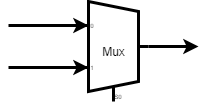
\includegraphics[width=0.2\textwidth]{fig-mux.png}
        \caption{数据选择器的电路模型}
        \label{fig:mux}
    \end{figure}

\subsection{指令内存模块(InstMem)}
    本实验中处理器采用哈佛架构,指令内存与数据内存分离。指令内存模块(InstMem)接受一个32位地址输入,输出一条32位指令。

\subsection{PC寄存器模块}
    PC寄存器模块用于管理PC地址。接受输入pcIn,在时钟上升沿将pcIn保存进PC寄存器。输出pcOut为当前PC地址,pcOut与PC寄存器内容即时同步。当reset信号处于高电平时,将PC值重置为0。

\subsection{顶层模块(top)}\label{sec:design-top}
    顶层模块将以上所有模块连接在一起,完成单周期CPU的功能。顶层模块中的连线包括数据通路和控制通路。数据通路用于传输中间数据,一般为32位或16位;控制通路用于传输控制信号。\par
    顶层模块主要的数据通路与控制通路如图\ref{fig:top}所示。图\ref{fig:top}来自于计算机系统结构课程(CS359)课件,特此向授课教师邓倩妮老师表示感谢。\par
    \begin{figure}[H]
        \centering
        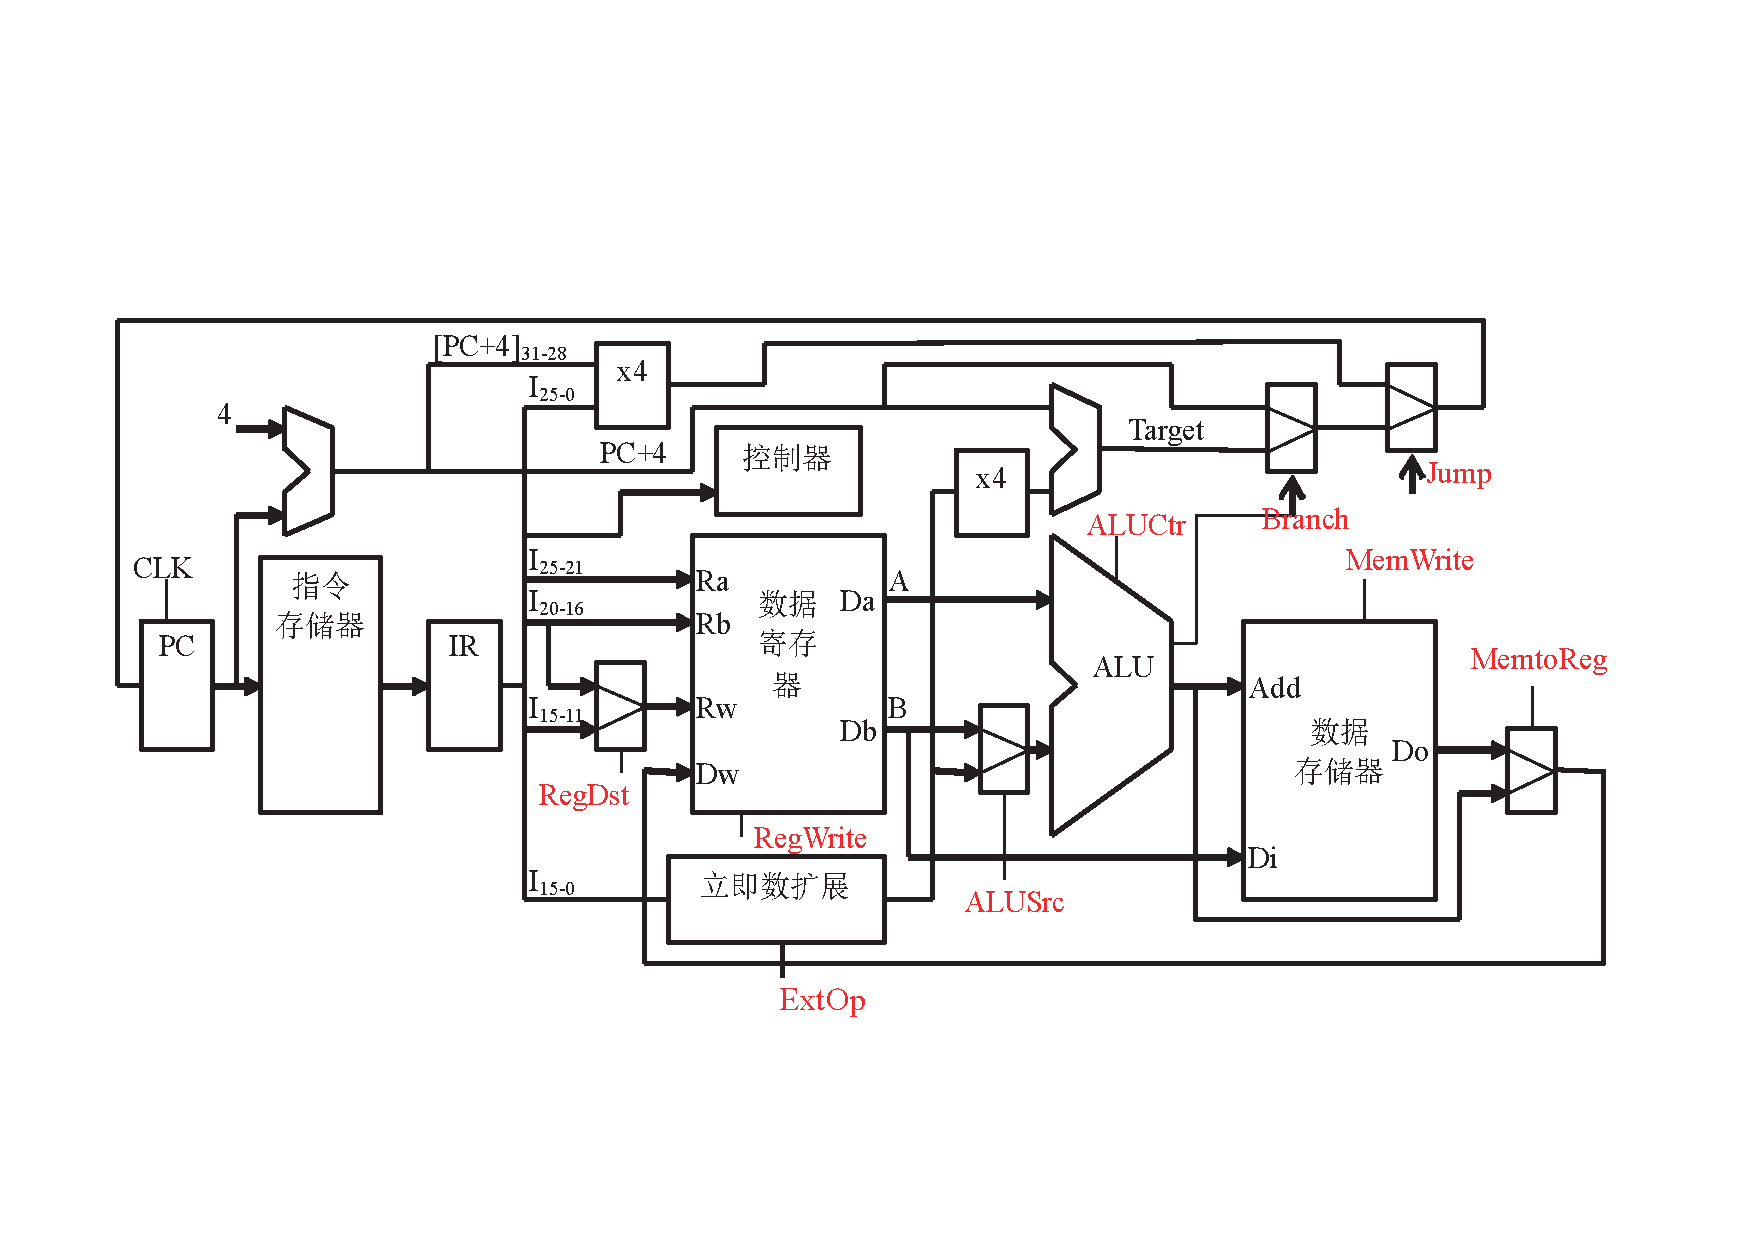
\includegraphics[width=0.9\textwidth]{fig-top.pdf}
        \caption{顶层模块基础数据通路与控制通路}
        \label{fig:top}
    \end{figure}
    在图\ref{fig:top}中,我们使用两个数据选择器用于选择下一个$PC$值,分别对应beq和j指令。对于非跳转指令,$PC+4$将被返回至PC寄存器模块。\par
    除图\ref{fig:top}中所示的基础通路外,我还添加了部分元件用于支持jal与jr指令。具体改动如下:
    \begin{itemize}
        \item 添加两个数据选择器用于选择写入寄存器编号与寄存器写入数据,以此完成jal指令的实现。处理jal指令时,jalSign信号与regWrite信号处于高电平,31号寄存器被选中,同时寄存器写数据端口输入$PC+4$。
        \item 在branch与jump选择器之间插入jr选择器,以此完成jr指令的实现。处理jr指令时,jrSign信号处于高电平,jr选择器选择寄存器读取结果,同时由于jump信号处于低电平,寄存器读取结果最终被返回至PC寄存器模块。
    \end{itemize}
    

\section{功能实现}\label{sec2}

\subsection{主控制器模块的实现}
本实验中,主控制器模块(Ctr)的输出结果由指令中opCode段决定。通过case语句,我们可以将指令与opCode对应,并根据每个指令的操作需求输出控制信号。\par
主控制器模块的完整实现见Ctr.v,本实验中实现相比实验3添加了部分控制信号并将ALUOp拓展为3位,其余部分与实验3中实现类似。部分核心代码如下:
\begin{lstlisting}[language=verilog]
always @(opCode)
begin
    case(opCode)
    6'b000000: //R type
    begin
        RegDst = 1;
        ALUSrc = 0;
        MemToReg = 0;
        RegWrite = 1;
        MemRead = 0;
        MemWrite = 0;
        Branch = 0;
        ExtSign = 0;
        JalSign = 0;
        ALUOp = 3'b101;
        Jump = 0;
    end
    6'b100011: //lw
    begin
        RegDst = 0;
        ALUSrc = 1;
        MemToReg = 1;
        RegWrite = 1;
        MemRead = 1;
        MemWrite = 0;
        Branch = 0;
        ExtSign = 1;
        JalSign = 0;
        ALUOp = 3'b000;
        Jump = 0;
    end
    //后续代码类似,此处省略
    endcase
end
\end{lstlisting}
受限于篇幅,此处只展示R型指令与lw指令对应的实现。\par
代码中RegDst、ALUSrc、MemToReg等为控制信号寄存器,与对应输出信号线相连。

\subsection{ALU控制器模块的实现}
ALU控制器模块(ALUCtr)的输出由aluOp与funct共同决定,其行为与主控制器模块(Ctr)相似。不同的是,aluOp与funct有部分位在部分指令中属于无关的位,因此我们使用casex替代case。casex中,可以用x表示我们不关心的位。\par
ALU控制器模块的完整实现见ALUCtr.v,相比实验3中实现,本实验的实现拓展了支持的运算类型,同时对ALUOp重新进行了编排。核心代码如下:
\begin{lstlisting}[language=verilog]
always @ (aluOp or funct)
begin
    ShamtSign = 0;
    JrSign = 0;
    casex({aluOp,funct})
        9'b000xxxxxx:  // lw,sw,add,addiu
            ALUCtrOut = 4'b0010;
        9'b001xxxxxx:  // beq
            ALUCtrOut = 4'b0110;
        9'b010xxxxxx:   //stli
            ALUCtrOut = 4'b0111;
        9'b110xxxxxx:   //stliu
            ALUCtrOut = 4'b1000;
        9'b011xxxxxx:  // andi
            ALUCtrOut = 4'b0000;
        9'b100xxxxxx:  // ori
            ALUCtrOut = 4'b0001;
        9'b111xxxxxx:  // xori
            ALUCtrOut = 4'b1011;
        9'b101001000:  // jr
        begin
            ALUCtrOut = 4'b0101;
            JrSign = 1;
        end
        //R type
        9'b101000000:  // sll
        begin
            ALUCtrOut = 4'b0011;
            ShamtSign = 1;
        end
        9'b101000010:  // srl
        begin
            ALUCtrOut = 4'b0100;
            ShamtSign = 1;
        end
        9'b101000011:  // sra
        begin
            ALUCtrOut = 4'b1110;
            ShamtSign = 1;
        end
        9'b101000100:  // sllv
            ALUCtrOut = 4'b0011;
        9'b101000110:  // srlv
            ALUCtrOut = 4'b0100;
        9'b101000111:  // srav
            ALUCtrOut = 4'b1110;

        9'b101100000:  // add
            ALUCtrOut = 4'b0010;
        9'b101100001:  // addu
            ALUCtrOut = 4'b0010;
        9'b101100010:  // sub
            ALUCtrOut = 4'b0110;
        9'b101100011:  // subu
            ALUCtrOut = 4'b0110;
        9'b101100100:  // and
            ALUCtrOut = 4'b0000;
        9'b101100101:  // or
            ALUCtrOut = 4'b0001;
        9'b101100110:  // xor
            ALUCtrOut = 4'b1011;
        9'b101100111:  // nor
            ALUCtrOut = 4'b1100;
        9'b101101010:  // slt
            ALUCtrOut = 4'b0111;
        9'b101101011:  // sltu
            ALUCtrOut = 4'b1000;
    endcase
end
\end{lstlisting}

\subsection{ALU模块的实现}
ALU模块根据aluCtr信号完成指定的功能,可以使用case语句选择操作,利用verilog自带的运算符完成运算。\par
ALU模块的完整实现见ALU.v,核心代码如下:
\begin{lstlisting}[language=verilog]
always @ (input1 or input2 or aluCtr)
begin
    case(aluCtr)
    4'b0000:    //AND
        ALURes = input1 & input2;
    4'b0001:    //OR
        ALURes = input1 | input2;
    4'b0010:    //ADD
        ALURes = input1 + input2;
    4'b0011:    //Left-shift
        ALURes = input2 << input1;
    4'b0100:    //Right-shift
        ALURes = input2 >> input1;
    4'b0101:
        ALURes = input1;
    4'b0110:    //SUB
        ALURes = input1 - input2;
    4'b0111:    //SLT
        ALURes = ($signed(input1) < $signed(input2));
    4'b1000:    //SLTU
        ALURes = (input1 < input2);
    4'b1011:    //xor
        ALURes = input1 ^ input2;
    4'b1100:    //nor
        ALURes = ~(input1 | input2);
    4'b1110:    //Right-shift-arithmetic
        ALURes = ($signed(input2) >> input1);
    endcase
    if(ALURes==0)
        Zero = 1;
    else
        Zero = 0;
end
\end{lstlisting}\par
SLT运算功能的实现中,由于Verilog会默认以无符号数解释wire类型,需要通过\$signed关键词将输入解释为带符号数后再进行比较。\par
在ALU模块的结尾,我们判断运算结果是否为0,并以此设置Zero寄存器,最终作为zero信号输出。

\subsection{寄存器模块的实现}
寄存器会一直进行读操作,而由regWrite控制写操作。为实现信号同步,保证信号的完整性,写操作仅在时钟下降沿进行。由于读操作即时进行,寄存器内容被修改后,对应寄存器的读取结果也会同时更新。\par
相比与实验4中的实现,本实验中寄存器模块可以响应reset信号,当reset为高电平时,所有寄存器清零。\par
寄存器模块的完整实现见Registers.v,核心部分代码如下:
\begin{lstlisting}[language=verilog]
reg [31:0] RegFile[31:0];
integer i;

initial begin
    RegFile[0] = 0;
end

assign readData1 = RegFile[readReg1];
assign readData2 = RegFile[readReg2];

always @ (negedge clk or reset)
begin
    if(reset)
    begin
        for(i=0;i<32;i=i+1)
            RegFile[i] = 0;
    end
    else begin
        if(regWrite)
            RegFile[writeReg] = writeData; 
    end
end
\end{lstlisting}

\subsection{内存单元模块的实现}
内存模块由memRead控制是否进行读取操作,当memRead或address信号发生变化或时钟处于下降沿时,内存模块会根据address指定的内存地址内容更新数据读取数据,并将其作为结果输出。尽管在实际的计算机系统中,内存写操作和内存读操作不会同时进行,但是本模块依然具备同时写与读的能力。\par
写操作由memWrite信号控制。与寄存器模块相似,为实现信号同步,保证信号的完整性,写操作仅在时钟下降沿进行。\par
内存模块的完整实现见dataMemory.v,核心部分代码如下:
\begin{lstlisting}[language=verilog]
reg [31:0] memFile [0:1023];
reg [31:0] ReadData;
always @(memRead or address) 
begin
    if(memRead)
    begin
        if(address<1023)
            ReadData = memFile[address];
        else
            ReadData = 0;
    end
end

always @(negedge clk)
begin
    if(memWrite)
        if(address<1023)
            memFile[address] = writeData;
    if(memRead)
        if(address<1023)
            ReadData = writeData;
end

assign readData = ReadData;
\end{lstlisting}
\subsection{带符号扩展模块的实现}
    带符号扩展可以通过在高16位填入立即数第15位实现,无符号扩展可以通过在高16位填入0实现。为了在两种工作模式下切换,可以通过一个三目运算符根据signExt信号在两种扩展结果中进行选择。\par
    带符号扩展模块的完整实现见signext.v,核心部分代码如下:
\begin{lstlisting}[language=verilog]
assign data = signExt?{{16{inst[15]}},inst[15:0]}:{{16{0}},inst[15:0]};
\end{lstlisting}

\subsection{数据选择器模块的实现}
    使用Verilog自带的三目运算符即可实现数据选择器的功能。Mux与RegMux的差异仅在于输入输出数据长度不同。\par
    数据选择器模块的完整实现见Mux.v与RegMux.v,核心代码如下:
\begin{lstlisting}[language=verilog]
assign out = select?input1:input0;
\end{lstlisting}

\subsection{指令内存模块的实现}
    指令内存模块只需要根据PC地址输出对应的指令,实现相对简单。\par
    指令内存模块的完整实现见InstMem.v,核心代码如下:
\begin{lstlisting}[language=verilog]
reg [31:0] instFile[0:1023];
assign inst = instFile[address/4];
\end{lstlisting}

\subsection{PC寄存器模块的实现}
    PC寄存器模块在时钟上升沿将pcIn保存进PC寄存器,同时保证pcOut输出与PC寄存器内容一致。\par
    PC寄存器模块的完整实现见PC.v,核心代码如下:
\begin{lstlisting}[language=verilog]
reg [31:0] PC;

initial PC = 0;

always @ (posedge clk or reset)
begin
    if(reset)
        PC = 0;
    else
        PC = pcIn;
end
assign pcOut = PC;
\end{lstlisting}

\subsection{顶层模块的实现}
顶层模块的原理如\ref{sec:design-top}节所述。为实现顶层模块,首先需要声明需要的所有连接线路。连线的声明如下:\par
\begin{lstlisting}[language=verilog]
wire REG_DST;
wire REG_WRITE;
wire EXT_OP;
wire ALU_SRC;
wire[2:0] ALU_OP;
wire[3:0] ALU_CTR;
wire BRANCH;
wire JUMP;
wire JAL_SIGN;
wire MEM_WRITE;
wire MEM_READ;
wire MEM_TO_REG;
wire ALU_ZERO;
wire SHAMT_SIGN;
wire JR_SIGN;
wire[4:0] WRITE_REG_ID;
wire[4:0] WRITE_REG_ID_AFTER_JAL_MUX;

wire[31:0] INST;
wire[31:0] REG_WRITE_DATA_AFTER_JAL_MUX;
wire[31:0] REG_WRITE_DATA;
wire[31:0] REG_READ_DATA1;
wire[31:0] REG_READ_DATA2;
wire[31:0] EXT_IMM;
wire[31:0] ALU_INPUT1;
wire[31:0] ALU_INPUT2;
wire[31:0] ALU_OUTPUT;
wire[31:0] MEM_OUTPUT_DATA;
wire[31:0] MEM_INPUT_DATA;
wire[31:0] PC_IN;
wire[31:0] PC_OUT;
wire[31:0] PC_AFTER_BRANCH_MUX;
wire[31:0] PC_AFTER_JR_MUX;
wire[31:0] JUMP_ADDR;
\end{lstlisting}\par
上述代码中,第一部分为控制信号连线,第二部分为数据通路连线。\par
除了将上述连线与各个模块的对应端口相连,还需要完成外部信号reset和clk的连接。reset与PC寄存器模块、寄存器模块相连,用于完成处理器重置工作;clk与PC寄存器模块、寄存器模块、数据内存模块相连,用于同步数据写入的时间。\par
以主控制器模块为例,其连接如下:
\begin{lstlisting}[language=verilog]
Ctr main_ctr(
    .opCode(INST[31:26]),
    .regDst(REG_DST),
    .aluSrc(ALU_SRC),
    .memToReg(MEM_TO_REG),
    .regWrite(REG_WRITE),
    .memRead(MEM_READ),
    .memWrite(MEM_WRITE),
    .branch(BRANCH),
    .aluOp(ALU_OP),
    .jump(JUMP),
    .extSign(EXT_OP),
    .jalSign(JAL_SIGN)
);
\end{lstlisting}\par
顶层模块中完成下一个PC地址选择部分的实现如下:
\begin{lstlisting}[language=verilog]
Mux branch_mux(
    .select(BRANCH & ALU_ZERO),
    .input1(PC_OUT+4+(EXT_IMM<<2)),
    .input0(PC_OUT+4),
    .out(PC_AFTER_BRANCH_MUX)
);

Mux jr_mux(
    .select(JR_SIGN),
    .input0(PC_AFTER_BRANCH_MUX),
    .input1(REG_READ_DATA1),
    .out(PC_AFTER_JR_MUX)
);

Mux jump_mux(
    .select(JUMP),
    .input0(PC_AFTER_JR_MUX),
    .input1(JUMP_ADDR),
    .out(PC_IN)
);
\end{lstlisting}\par
顶层模块中jal指令相关数据选择器的连线如下:
\begin{lstlisting}[language=verilog]
Mux jal_data_mux(
    .select(JAL_SIGN),
    .input0(REG_WRITE_DATA),
    .input1(PC_OUT+4),
    .out(REG_WRITE_DATA_AFTER_JAL_MUX)
);

Mux jal_reg_id_mux(
    .select(JAL_SIGN),
    .input0(WRITE_REG_ID),
    .input1(5'b11111),
    .out(WRITE_REG_ID_AFTER_JAL_MUX)
);
\end{lstlisting}\par
其中REG\_WRITE\_DATA\_AFTER\_JAL\_MUX与寄存器模块的writeData端口相连,\\WRITE\_REG\_ID\_AFTER\_JAL\_MUX与寄存器模块的writeReg端口相连。\par
顶层模块的完整实现见top.v。

\section{结果验证}
编写如表\ref{tab:sim-inst}所示的汇编代码进行测试。\par
% Please add the following required packages to your document preamble:
% \usepackage{multirow}
% \usepackage{longtable}
% Note: It may be necessary to compile the document several times to get a multi-page table to line up properly
\begin{longtable}[c]{|c|c|c|p{1.5cm}<{\centering}|p{1.5cm}<{\centering}|p{1.5cm}<{\centering}|}
    \hline
    \multirow{2}{*}{地址} & \multirow{2}{*}{指令} & \multirow{2}{*}{汇编指令} & \multicolumn{3}{c|}{执行结果} \\ \cline{4-6} 
     &  &  &  \$0  &  \$1 & \$2 \\ \hline
    \endfirsthead
    %
    \endhead
    %
    0x00 & 00001000000000000000000000000100 & j & \multicolumn{3}{c|}{跳转至0x10} \\ \hline
    0x04 & 00000000000000000000000000000000 & nop & \multicolumn{3}{c|}{不执行} \\ \hline
    0x08 & 00000000000000000000000000000000 & nop & \multicolumn{3}{c|}{不执行} \\ \hline
    0x0c & 00000000000000000000000000000000 & nop & \multicolumn{3}{c|}{不执行} \\ \hline
    0x10 & 00001100000000000000000000000110 & jal & \multicolumn{3}{c|}{跳转至0x18, \$31 = 0x14} \\ \hline
    0x14 & 00000000000000000000000000000000 & nop & \multicolumn{3}{c|}{空指令} \\ \hline
    0x18 & 10001100000000010000000000000011 & lw $1,3($0) & 3 & x & x \\ \hline
    0x1c & 10001100000000100000000000000100 & lw $2,4($0) & 3 & 4 & x \\ \hline
    0x20 & 00000000001000100001100000100000 & add $3,$1,\$2 & 3 & 4 & 7 \\ \hline
    0x24 & 00000000001000100001100000100100 & and $3,$1,\$2 & 3 & 4 & 0 \\ \hline
    0x28 & 00000000001000100010000000100010 & sub $4,$1,\$2 & \multicolumn{3}{c|}{\$4 = -1} \\ \hline
    0x2c & 00000000000000010000100001000000 & sll $1,$1,1 & 6 & 4 & 0 \\ \hline
    0x30 & 00000000000000110001100011000000 & sll $3,$3,3 & 6 & 4 & 0 \\ \hline
    0x34 & 00000000001000110000100000100101 & or $1,$3,\$1 & 6 & 4 & 0 \\ \hline
    0x38 & 00100000000000100000000000000110 & addi $2,$0,6 & 6 & 6 & 0 \\ \hline
    0x3c & 00101000010000010000000000000001 & slti $1,$1,1 & 0 & 6 & 0 \\ \hline
    0x40 & 00110100010000010000000000000001 & ori $1,$2,1 & 7 & 6 & 0 \\ \hline
    0x44 & 00000000010000110000100000000100 & sllv $1,$3,\$2 & 0 & 6 & 0 \\ \hline
    0x48 & 00000000001000100001100000100001 & addu $3,$1,\$2 & 0 & 6 & 6 \\ \hline
    0x4c & 00000000001000100001100000100010 & sub $3,$1,\$2 & 0 & 6 & -6 \\ \hline
    0x50 & 00000000001000100001100000100011 & subu $3,$1,\$2 & 0 & 6 & -6 \\ \hline
    0x54 & 00000000001000100001100000100101 & or $3,$1,\$2 & 0 & 6 & 6 \\ \hline
    0x58 & 00000000001000100001100000100110 & xor $3,$1,\$2 & 0 & 6 & 6 \\ \hline
    0x5c & 00000000001000100001100000100111 & nor $3,$1,\$2 & 0 & 6 & -7 \\ \hline
    0x60 & 00000000001000100001100000101010 & slt $3,$1,\$2 & 0 & 6 & 1 \\ \hline
    0x64 & 00000000000000010000100001000011 & sra $1,$1,1 & 0 & 6 & 1 \\ \hline
    0x68 & 10101100000000100000000000000001 & sw $2,1($0) & \multicolumn{3}{c|}{写入内存} \\ \hline
    0x6c & 00010000101000000000000000000001 & beq $5,$0,1 & \multicolumn{3}{c|}{跳转至0x74} \\ \hline
    0x70 & 00000000010000000000000000001000 & jr \$2 & \multicolumn{3}{c|}{不执行} \\ \hline
    0x74 & 00000011111000000000000000001000 & jr \$31 & \multicolumn{3}{c|}{跳转至0x14} \\ \hline
    \caption{仿真使用的指令}
    \label{tab:sim-inst}\\
    \end{longtable}
    数据内存的初始值如表\ref{tab:sim-data}所示。\par
\begin{table}[htbp]
    \centering
    \begin{tabular}{|c|c|}
    \hline
    地址 & 数据 \\ \hline
    0x00 & 0x00000000 \\
    0x01 & 0x00000001 \\
    0x02 & 0x00000002 \\
    0x03 & 0x00000003 \\
    0x04 & 0x00000004 \\
    0x05 & 0x00000005 \\ \hline
    \end{tabular}
    \caption{数据内存初始值}
    \label{tab:sim-data}
    \end{table}
在激励文件中载入指令内存与数据内存数据。\par
\begin{lstlisting}[language=verilog]
$readmemb("E:/course/arclab/lab05/mem_inst.dat",top.inst_mem.instFile);
$readmemh("E:/course/arclab/lab05/mem_data.dat",top.memory.memFile);
\end{lstlisting}\par
仿真结果如图\ref{fig:sim-res}所示。需要特别说明的是,由于显示缩放问题,部分数字可能没有显示完整。
\begin{figure}[H]
    \centering
    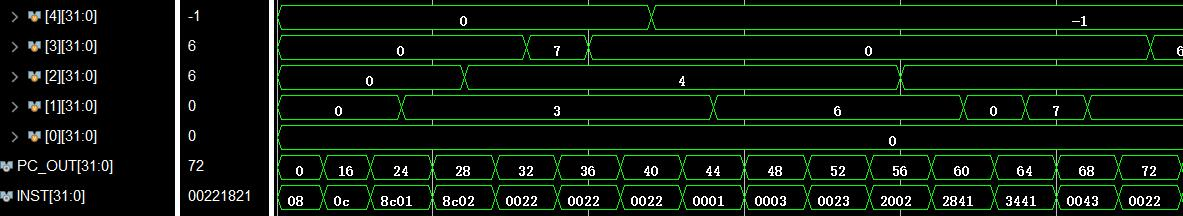
\includegraphics[width=\textwidth]{fig-lab5-sim1.jpg}
    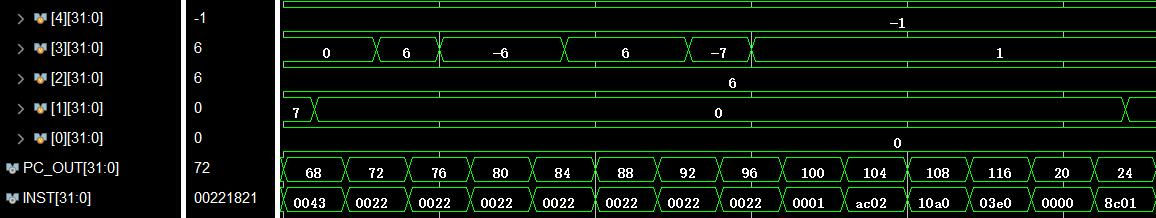
\includegraphics[width=\textwidth]{fig-lab5-sim2.jpg}
    \caption{仿真截图}
    \label{fig:sim-res}
\end{figure}\par
可以看出,我们实现的类MIPS单周期处理器完成了设计的所有功能。

\section{总结与反思}
本实验结合实验3和实验4实现的功能模块,实现了一个类MIPS单周期处理器。由于我们在计算机系统结构课程已经学习过单周期处理器结构,本实验的实现较为简单。本实验也让我明白,在计算机系统中,想实现一个复杂化的功能,只需要先实现所有简单模块再组合在一起即可。\par
本实验主要难度在于调试阶段,在初次实现顶层模块时,我没有作出连线图,而是凭借自己的记忆进行连线,出现了较多连线错误,导致调试工作异常复杂。最终,我按照计算机系统结构课程课件上提供的单周期处理器连线图重新检查了所有连线。这样的经历提醒我,在以后的实验中,应当先完成整体设计再开始代码实现。\par
除此之外,为编写本次实验中用于仿真的代码,我复习了MIPS指令的相关知识,重新熟悉了MIPS指令的分类、分段结构。\par
总而言之,本次实验让我受益匪浅。
\end{document}